\documentclass{cslthse-msc}
\usepackage[utf8]{inputenc}
\usepackage[english]{babel}
\usepackage{amsmath}
\usepackage{amsfonts}
\usepackage{amssymb}
\usepackage{amsthm}
%\usepackage{makeidx}
\usepackage{graphicx}
\usepackage[titletoc, header, page]{appendix}

\usepackage{hyperref}
\usepackage{pdfpages}
\usepackage{rotating}
\usepackage{enumitem}
\usepackage{subfig}
\usepackage{float}
\usepackage{listings}
\input{listings-modelica.cfg}

%\geometry{showframe}

\author{
	Erik Hedblom \\
	{\normalsize \href{mailto:hedblom.e@gmail.com}{\texttt{hedblom.e@gmail.com}}}
	\and
	Kasper Rundquist \\
	{\normalsize \href{mailto:kasper.rundquist@gmail.com}{\texttt{kasper.rundquist@gmail.com}}}
}

\title{Safe regression test selection using static analysis}
%\subtitle{A {\LaTeX} class}
\company{Modelon AB}
\supervisors{Johan Ylikiiskilä, \href{mailto:johan.ylikiiskila@modelon.com}{\texttt{johan.ylikiiskila@modelon.com}}}{Jonatan Kämpe, \href{mailto:jonathan.kampe@modelon.com}{\texttt{jonathan.kampe@modelon.com}}}{Niklas Fors, \href{mailto:niklas.fors@cs.lth.se}{\texttt{niklas.fors@cs.lth.se}}}%\supervisor{Niklas Fors, \href{mailto:niklas.fors@cs.lth.se}{\texttt{niklas.fors@cs.lth.se}}}
\examiner{Görel Hedin, \href{mailto:gorel.hedin@cs.lth.se}{\texttt{gorel.hedin@cs.lth.se}}}

\date{\today}
%\date{January 16, 2015}

\acknowledgements{
If you want to thank people, do it here, on a separate right-hand page. Both the U.S. \textit{acknowledgments} and the British \textit{acknowledgements} spellings are acceptable.
}

\theabstract{
This document describes the Master's Thesis format for the theses carried out at 
the Department of Computer Science, Lund University. 

Your abstract should capture, in English, the whole thesis with focus on the problem and solution in 150 words. It should be placed on a separate right-hand page, with an additional \textit{1cm} margin on both left and right. Avoid acronyms, footnotes, and references in the abstract if possible.

Leave a \textit{2cm} vertical space after the abstract and provide a few keywords relevant for your report. Use five to six words, of which at most two should be from the title.
}

\keywords{Test Selection, Modelica}

\divisionoflabor{
}

%% Only used to display font sizes
\makeatletter
\newcommand\thefontsize[1]{{#1 \f@size pt\par}}
\makeatother
%%%%%%%%%%


\begin{document}
\makefrontmatter
\chapter[Introduction]{Introduction}

\section{Motivation / Background}
During software development, when a change is integrated into a project all previous testing have to be rerun. Test suites usually accumulates over time and regression testing can therefore be very time consuming. Depending on the change some or most of the test may be unrelated to the change and by excluding unrelated tests significant time savings could be achieved. ~\cite{DUMMY}


Det är viktig att testa mjukvara under utvecklingen för säkerställa att mjukvaran fungerar korrekt. När mjukvaran uppdateras måste testfall som redan testats utföras igen för att kontrollera att allt som fungerade innan uppdatering fortfarande fungerar efter. Det kan vara väldigt tidskrävande att köra samtliga test. Det finns därför mycket tid att spara om det går att utesluta test som garanterat inte har påverkas. För språket Modelica finns det inget verktyg för detta och det är därför intressant att utveckla ett.

\section{Problem Description / Aim / Goal}

The aim of this project is too reduce testing times for Modelica projects without loss of quality. This will be done by developing and implementing a method to exclude tests in a test suite unaffected by a specific change. Regression testing can then be performed with a reduced test suite without compromising quality.

\section{Regression Testing}
Regression tests are used to make sure that regression dose not occur. Software regression is when something that did work before do not work as expected due to a change.

\chapter[Background]{Background}

\section{Model Testing Toolkit}
Model testing Toolkit, MTT, is based on nose tests for Python \cite{noseDoc}. Nose finds all tests automatically and runs them if nothing is specified. In MTT a test case is represented by a xml file and every test case has a Modelica model. So when you like to run test cases only associated with a specific model it's easy to select only the test cases which have the model you are interested in.

When tests are run in MTT a HTML report of the results are created.

\section{Test Selection}
\begin{itemize}
	\item What is test selection?
	\item Different approaches
\end{itemize}
A safe Regression Test Selection (RTS) method will select all tests that produce a new result after a specific change. A safe RTS method is equivalent to running all tests. For a RTS method to be useful the RTS algorithm should run in less time than it takes to run the excluded tests. This is not necessary for each run, on average the overhead needs to be less than the time it takes to run the excluded tests.


\section{Modelica}
\begin{itemize}
	\item What is Modelica?
	\item How can we perform test selection for Modelica?
	\item SourceTree, InstanceTree, FlatTree
	\end{itemize}

\subsection{Classes}
Basically everything in Modelica is classes. Built in types such as Integer are Modelica classes. Packages, models and functions are classes. Modelica is an object-oriented language, inheritance is possible. The extends clause is used to create an subclass of an superclass. In figure \ref{fig:classDefinition}, P2 is a subclass to P1, which is a superclass to P2. The subclass inherits everything in the superclass. The subclass may have more content than the superclass, but all the content in the super class is also in the subclass. 

\begin{figure}[H]
    \centering
    \subfloat{{\lstinputlisting[language=modelica]{modelica/packageDecl.mo}}}
    \caption{Class definition}
    \label{fig:classDefinition}
\end{figure}

A redeclare can be used to replace the declaration of an class or component with a new declaration. A component is a variable or an instance of a class. In figure ~\ref{fig:redeclare}, x is declared in model A. An instance of A is created in model C where x is redeclared. The y in model B, B.y, will have the value 1, while the y in model C, C.y, will have the value 2.

\begin{figure}[H]
	\lstinputlisting[language=modelica]{modelica/redeclare.mo}
    \caption{Redeclare}
    \label{fig:redeclare}
\end{figure}

\subsection{Import}
Imports are possible in Modelica to refer to a class or component in an other package. An import creates an alias. In the import below HydralicConductance will be mapped to the fully qualified name Modelica.Fluid.Types.HydralicConductance.

\lstinputlisting[language=modelica]{modelica/import.mo}

Modelica offers the option to rename an import. Here an alias will be created where the name Conductance is mapped to the fully qualified name Modelica.Fluid.Types.HydralicConductance.

\lstinputlisting[language=modelica]{modelica/renamedImport.mo}

Modelica allows the use of wildcard imports. Using wildcards it isn't possible to rename the import. This wildcard import will create an alias for every definition in Modelica.Fluid.

\lstinputlisting[language=modelica]{modelica/wildcardImport.mo}

To avoid multiple imports and wildcard imports, an multiple definition import can be used, from Modelica specification 3.3 \cite{modelicamodelica}. This multiple definition import creates two aliases, one mapping HydralicConductance to Modelica.Fluid.Types.HydralicConductance and one mapping HydralicResistance to Modelica.Fluid.Types.HydralicResistance.

\lstinputlisting[language=modelica]{modelica/multipleDefinitionImport.mo}

\subsection{Name lookup}
In order to find a match for a name, Modelica starts by looking at the first name in a qualified name. Take for example the fully qualified name Modelica.Fluid.Pipes.StaticPipe. In this example Modelica is the first name in the qualified name.

To find a match for the name, Modelica first checks if it's a built in type. If it's a built in type Modelica has found a match for the name.

If it's not a built in type Modelica looks in the class where the name is used, including inherited definitions, for a nested definition of the name. 

If there is no nested definition of the name, Modelica looks in the imports in the class where the name is used, inherited imports are not included, to find a match for the name.

If a match for the name is not found in the imports, Modelica looks for a nested definition in the parent package, including inherited definitions.

If the definition of the name isn't found in the parent package, Modelica looks for a imported definition, not including inherited imports, in the parent package.

If a match for the name still not is found, Modelica continues by using the same method and looking in the parent packages parent package and so on until: the parent package has the encapsulated qualifier or a package doesn't have a parent package. In the first case the search for the name terminates and in the second case Modelica searches for a match in root level packages.

The search is done in the same way for the first name in a qualified name and an unqualified name. An unqualified name doesn't contain a dot, an unqualified name consists of only one name. StaticPipe is an example of an unqualified name.

If a name is a part of a qualified name and isn't the first name in the qualified name, it must be a nested definition within the definition of the previous name in the qualified name. In the example Modelica.Fluid.Pipes.StaticPipe, Fluid must be a nested definition within Modelica.\cite{modelicamodelica, tillermodelica}

\subsection{Accesses}

\section{JastAdd}
JastAdd is a system based on reference attribute grammars, for extensible implementation of compilers. An Abstract Syntax Tree (AST) is used to represent a program. Attribute Grammars is amethod for declerativly defining computations on an AST. A node in an AST can have a synthezied attribute or an inherited attribute. An attribue is defined by an equation. A synthezied attribyte is defined in the node, an inherired attribute is defined in an ancestor node. A JastAdd specification is used to create an object-oriented framework.~\cite{aakesson2008development}

Collection attributes are defined by partial definitions in a number of arbitrary nodes. A node that have a partial definition of a collection attribute contributes to the value of the collection attribute. A collection attribute is usually a set where the empty set is the initial value of the collection attribute. The contributors, the nodes that contributes to the collection attribute, can for example contribute by adding elements to the set.~\cite{magnusson2007extending}

\chapter[Dependency analysis]{Dependency analysis}



\section{Dependency Rules}

To build the dependency graph we have constructed a set of rules to determine what creates dependencies. Due to limitations in JModelica mainly pertaining to the lookup of names in the source tree. The rules have been adjusted to work around these limitations. We hope to have time to fix the limitations to perform a better and more accurate dependency analysis. 

\begin{enumerate}
\item A class depends on its parent class. 
\item A class depends on all accesses within it.
\item A class depends on all classes in the paths of its accesses.
\item A class depends on all classes defined in an accessed class.
\item Exception of rule 4. A class doesn't depend on classes defined in an accessed class if the accessed class is accessed through an import.
\end{enumerate}

\section{Dependency analysis}

The dependency model we have developed have two types of dependencies, parent and access dependencies. Parent dependencies are dependencies that occur due to Modelicas lookup and scoping rules. This means that classes depend on the class they are defined in, their parent. This is handled by rule 1. Consider the following code:

\lstinputlisting[language=modelica]{modelica/parent1.mo}
\begin{figure}
    \centering
    \includegraphics[]{EPS-graphs/parent1.eps}
  \caption{The dependency graph}
  \label{fig:parent1graph}
\end{figure}

D has a dependency to A.k since it accesses the constant k. This is not a parent dependency and we will leave it for now. D also has dependencies to B and C due to Modelicas scoping and lookup rules. If k is redefined in either B or C, the reference to k in D will refer to k in C or B instead. To handle this type of dependency we say that a class has a dependency to its parent class.

Another way to think about it is to consider what happens if a parent is removed. The class can no longer be accessed since the path to it is broken. This will cause the compilation of the class to fail. The corresponding dependency graph is found in figure \ref{fig:parent1graph}.

Access dependencies are all the other dependencies, dependencies created by accesses. However, one access can create one, many or no dependencies. If an access have a path,s each part of the path creates a dependency. This is an example:
\lstinputlisting[language=modelica]{modelica/import1.mo}
The class E have an access P.A.B.D referring to P.C.D. The access also creates dependencies to P, P.A and P.A.B. If P, P.A or P.A.B is removed E will fail to build since the path P.A.B.D is broken. Another case to consider is if B redefines D, D in E will then have changed.





In figure \ref{fig:extends}, class C is the accessed class in the immediate subtree of class A. Class B is in the path to the accessed class. Class E is an subclass to class C.
Example:
\begin{figure}[H]
    \centering
    	\subfloat{{\includegraphics[scale=0.8]{EPS-graphs/extends.eps}}}
    	\qquad
    	\subfloat{\raisebox{4.5 cm}{\lstinputlisting[language=modelica]{modelica/extends.mo}}}
    \caption{Extends Graph}
    \label{fig:extends}
\end{figure}

\begin{figure}[H]
    \centering
    \subfloat{{\includegraphics[scale=0.8]{EPS-graphs/ParentExample.eps}}}
    \qquad
    \subfloat{\raisebox{3.2 cm}{\lstinputlisting[language=modelica]{modelica/parentExample.mo}}}
    \caption{Parent graph}
    \label{fig:parentGraph}
\end{figure}

There is a constant k defined in package A, in figure \ref{fig:parentGraph}. If we define a constant k in model B, the k accessed in C will be k defined in model B instead of the k defined in A. Therefore we need a dependency from C to B.

If the constant k in package A is changed it will affect model C. Therefore we need a dependency from C to A. With rule number 1 we get dependencies from C to B and from B to A. So we have an indirect dependency from C to A.

If the components or classes that is used in a class is changed it might change the behavior of that class. Thus we need rule number 2.

\begin{figure}[H]
    \centering
    \subfloat{{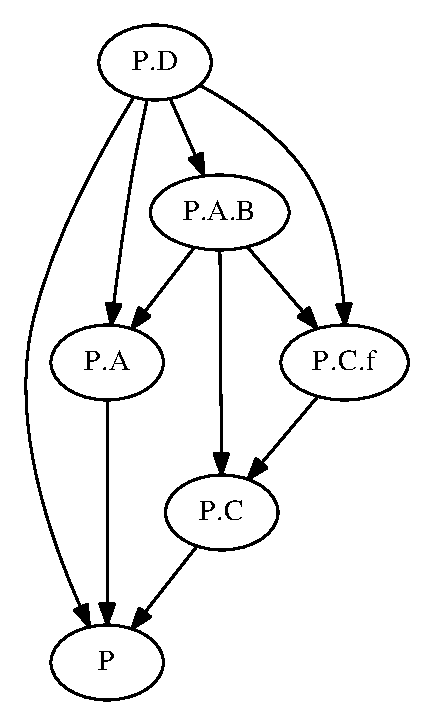
\includegraphics[scale=0.8]{EPS-graphs/DotAccess.eps}}}
    \qquad
    \subfloat{\raisebox{10 cm}{
    	\begin{minipage}[t]{.5\textwidth}
			\centering
			\lstinputlisting[language=modelica]{modelica/DotAccess.mo}
			\lstinputlisting[language=modelica]{modelica/DotAccessC.mo}
		\end{minipage}}}
    \caption{Dot Access}
    \label{fig:dotAccess}
\end{figure}

In figure \ref{fig:dotAccess}, we want dependencies from model D to all parts in the path of the access of f. The parts of the access of f is P.A, P.A.B and P.C.f. If package A or B is deleted it will cause a compilation error when  model D is compiled. This is way rule number 3 is needed.

\begin{figure}[H]
    \centering
    \subfloat{{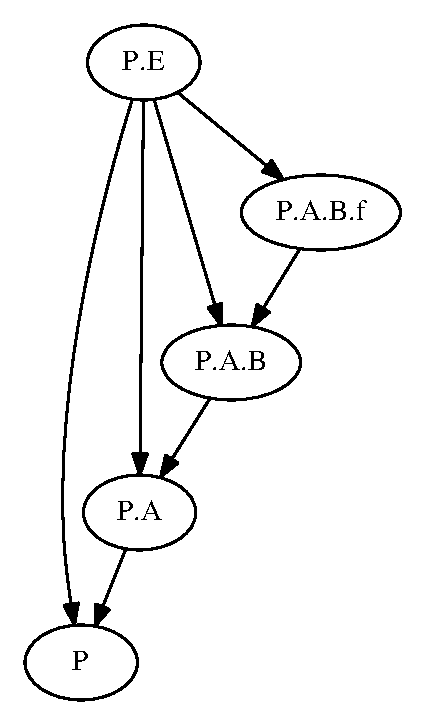
\includegraphics[scale=0.8]{EPS-graphs/GraphA.eps}}}
    \qquad
    \subfloat{\raisebox{4.7 cm}{\lstinputlisting[language=modelica]{modelica/exampleA.mo}}}
    \caption{Instantiation}
    \label{fig:instantiation}
\end{figure}

When we create an instance of A in model E, we want dependencies from E to A and everything in A, see figure \ref{fig:instantiation}. We want to have a dependency from E to the subtree with A as a root, in this case the subtree consists of the nodes P.A, P.A.B and P.A.B.f. This is because we are working in the source tree in the compiler and there's no functionality to lookup a, the instance of A. We can't find f in a.B.f. This is way rule number 4 is needed.

\begin{figure}[H]
    \centering
    \lstinputlisting[language=modelica]{modelica/importRootPackage.mo}
    \caption{Root package import}
    \label{fig:importRootPackage}
\end{figure}

If we look at figure \ref{fig:importRootPackage}, Modelica.Constants.pi could be accessed without first importing Modelica since the package Pipes, which Modelica.Constants.pi is used in, is in the same enclosing package as the package Constants.

But now we instead look at figure \ref{fig:newPackageWithoutImport}, where Modelica not is imported and there is a new package also named Modelica in the package Fluid. When the new package Modelica.Fluid.Modelica is added pi won't be found. When trying to lookup Modelica.Constants.pi the package Modelica.Fluid.Modelica will found and it doesn't contain a class with the name Constants, so the lookup will fail.

If Modelica had been imported the lookup of Modelica.Constants.pi had succeeded since an import starts at a root level package. This is the reason for the imports of the root package that are unnecessary at the moment but guarantees the right class or component always will be found. Even if someone in the future adds a new package with same name as an existing package.

\begin{figure}[H]
    \centering
    \lstinputlisting[language=modelica]{modelica/newPackageWithoutImport.mo}
    \caption{New package without import}
    \label{fig:newPackageWithoutImport}
\end{figure}

Handling imports as other accesses a lot of extra dependencies, and in case of imports it's not necessary to dependencies to classes defined in the imported class. And therefore we need rule number 5. In case of an import, the other rules makes sure that when something in the imported class is used we get a dependency to all the accessed classes. In figure \ref{fig:importRootPackage}, we get a dependency from Modelica.Fluid.Pipes to Modelica.Constants, not to all classes that might be in the package Modelica.


\subsection{Incremental updating}

\section{Test selection}

\chapter[Implementation]{Implementation}
We have implemented two different options for the dependency analysis, it can either be done based on files or Modelica classes. To do the dependency analysis and get an inverted dependency graph from the Modelica compiler, we specify which files or models that has changed. The dependency analysis are done for the specified Modelica classes or for all Modelica classes in the specified files. After the dependency analysis is done we invert the graph and returns a set of Modelica classes that may have changed.

If a class depends on something in, a library that aren't a part of any of the following: 
\begin{itemize}
	\item The library the class is in.
	\item The library any of the other specified classes are in.
	\item The library of, a class that are set to be included in the analysis
\end{itemize}
the dependency to that library is not included in the dependency graph. Lets look at an example where we specify that class P.A, in figure \ref{fig:libraryGraph}, has changed. Then P is the root library A is in. A have a dependency to B in library MSL, here we will not include MSL.B in the dependency analysis and by that neither classes that MSL.B depends on. When we find a dependency to MSL.B we stops the analysis there.

\begin{figure}[H]
    \centering
    \subfloat{{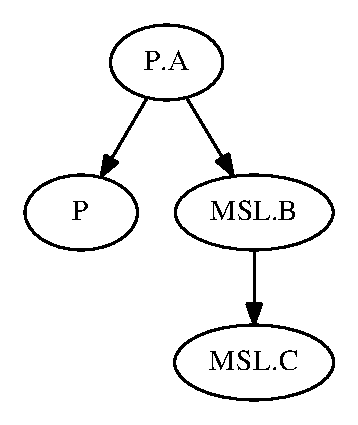
\includegraphics[scale=0.8]{EPS-graphs/LibraryExample.eps}}}
    \caption{Dependency graph}
    \label{fig:libraryGraph}
\end{figure}

Summary of approach:
\begin{itemize}
	\item Only do dependency analysis on given Modelica classes
	\item Don't continue the analysis in libraries that aren't specified
\end{itemize}
\section{Inverted dependency graph}
\begin{figure}[H]
    \centering
    \subfloat{{\includegraphics[scale=0.8]{EPS-graphs/GraphExample.eps}}}
    \caption{Dependency graph.}
    \label{fig:dependencyGraph}
\end{figure}
In the example above figure \ref{fig:dependencyGraph}, we have two Modelica classes, C1 and C2. C2 have a dependency to C1. We also have two tests, T1 and T2. T1 tests C1 and T2 tests C2. When C1 is changed both tests, T1 and T2 should be selected. When C2 is changed only test T2 needs to be selected.

When we specify that a class has changed, we want to get a set containing all classes that may be affected. So if we specify that C2 has changed, C2 is the only class that can be affected. If we instead say that C1 has changed both C1 and C2 may be affected. Starting from C1, the problem is to find all classes that depends on C1. To solve this we need to invert the dependency graph, in figure \ref{fig:dependencyGraph}, and then get the inverted dependency graph in figure \ref{fig:invertedGraph}. 
\begin{figure}[H]
    \centering
    \subfloat{{\includegraphics[scale=0.8]{EPS-graphs/InvertedGraphExample.eps}}}
    \caption{Inverted dependency graph.}
    \label{fig:invertedGraph}
\end{figure}
\section{External functions}
The Modelica language allows the use of external functions that are not defined in a Modelica file. The external functions are often defined in a C-file.\cite{modelicamodelica}

In our dependency analysis we can't analyze the dependencies in external files. To handle this, and keep the test selection safe, if a file that isn't a Modelica file has changed we assume that every Modelica class that has a reference to an external has changed.
\chapter[Evaluation]{Evaluation}
\begin{itemize}
	\item Savings
	\item Precision
\end{itemize}

\begin{figure}
    \centering
    \makebox[\textwidth][c]{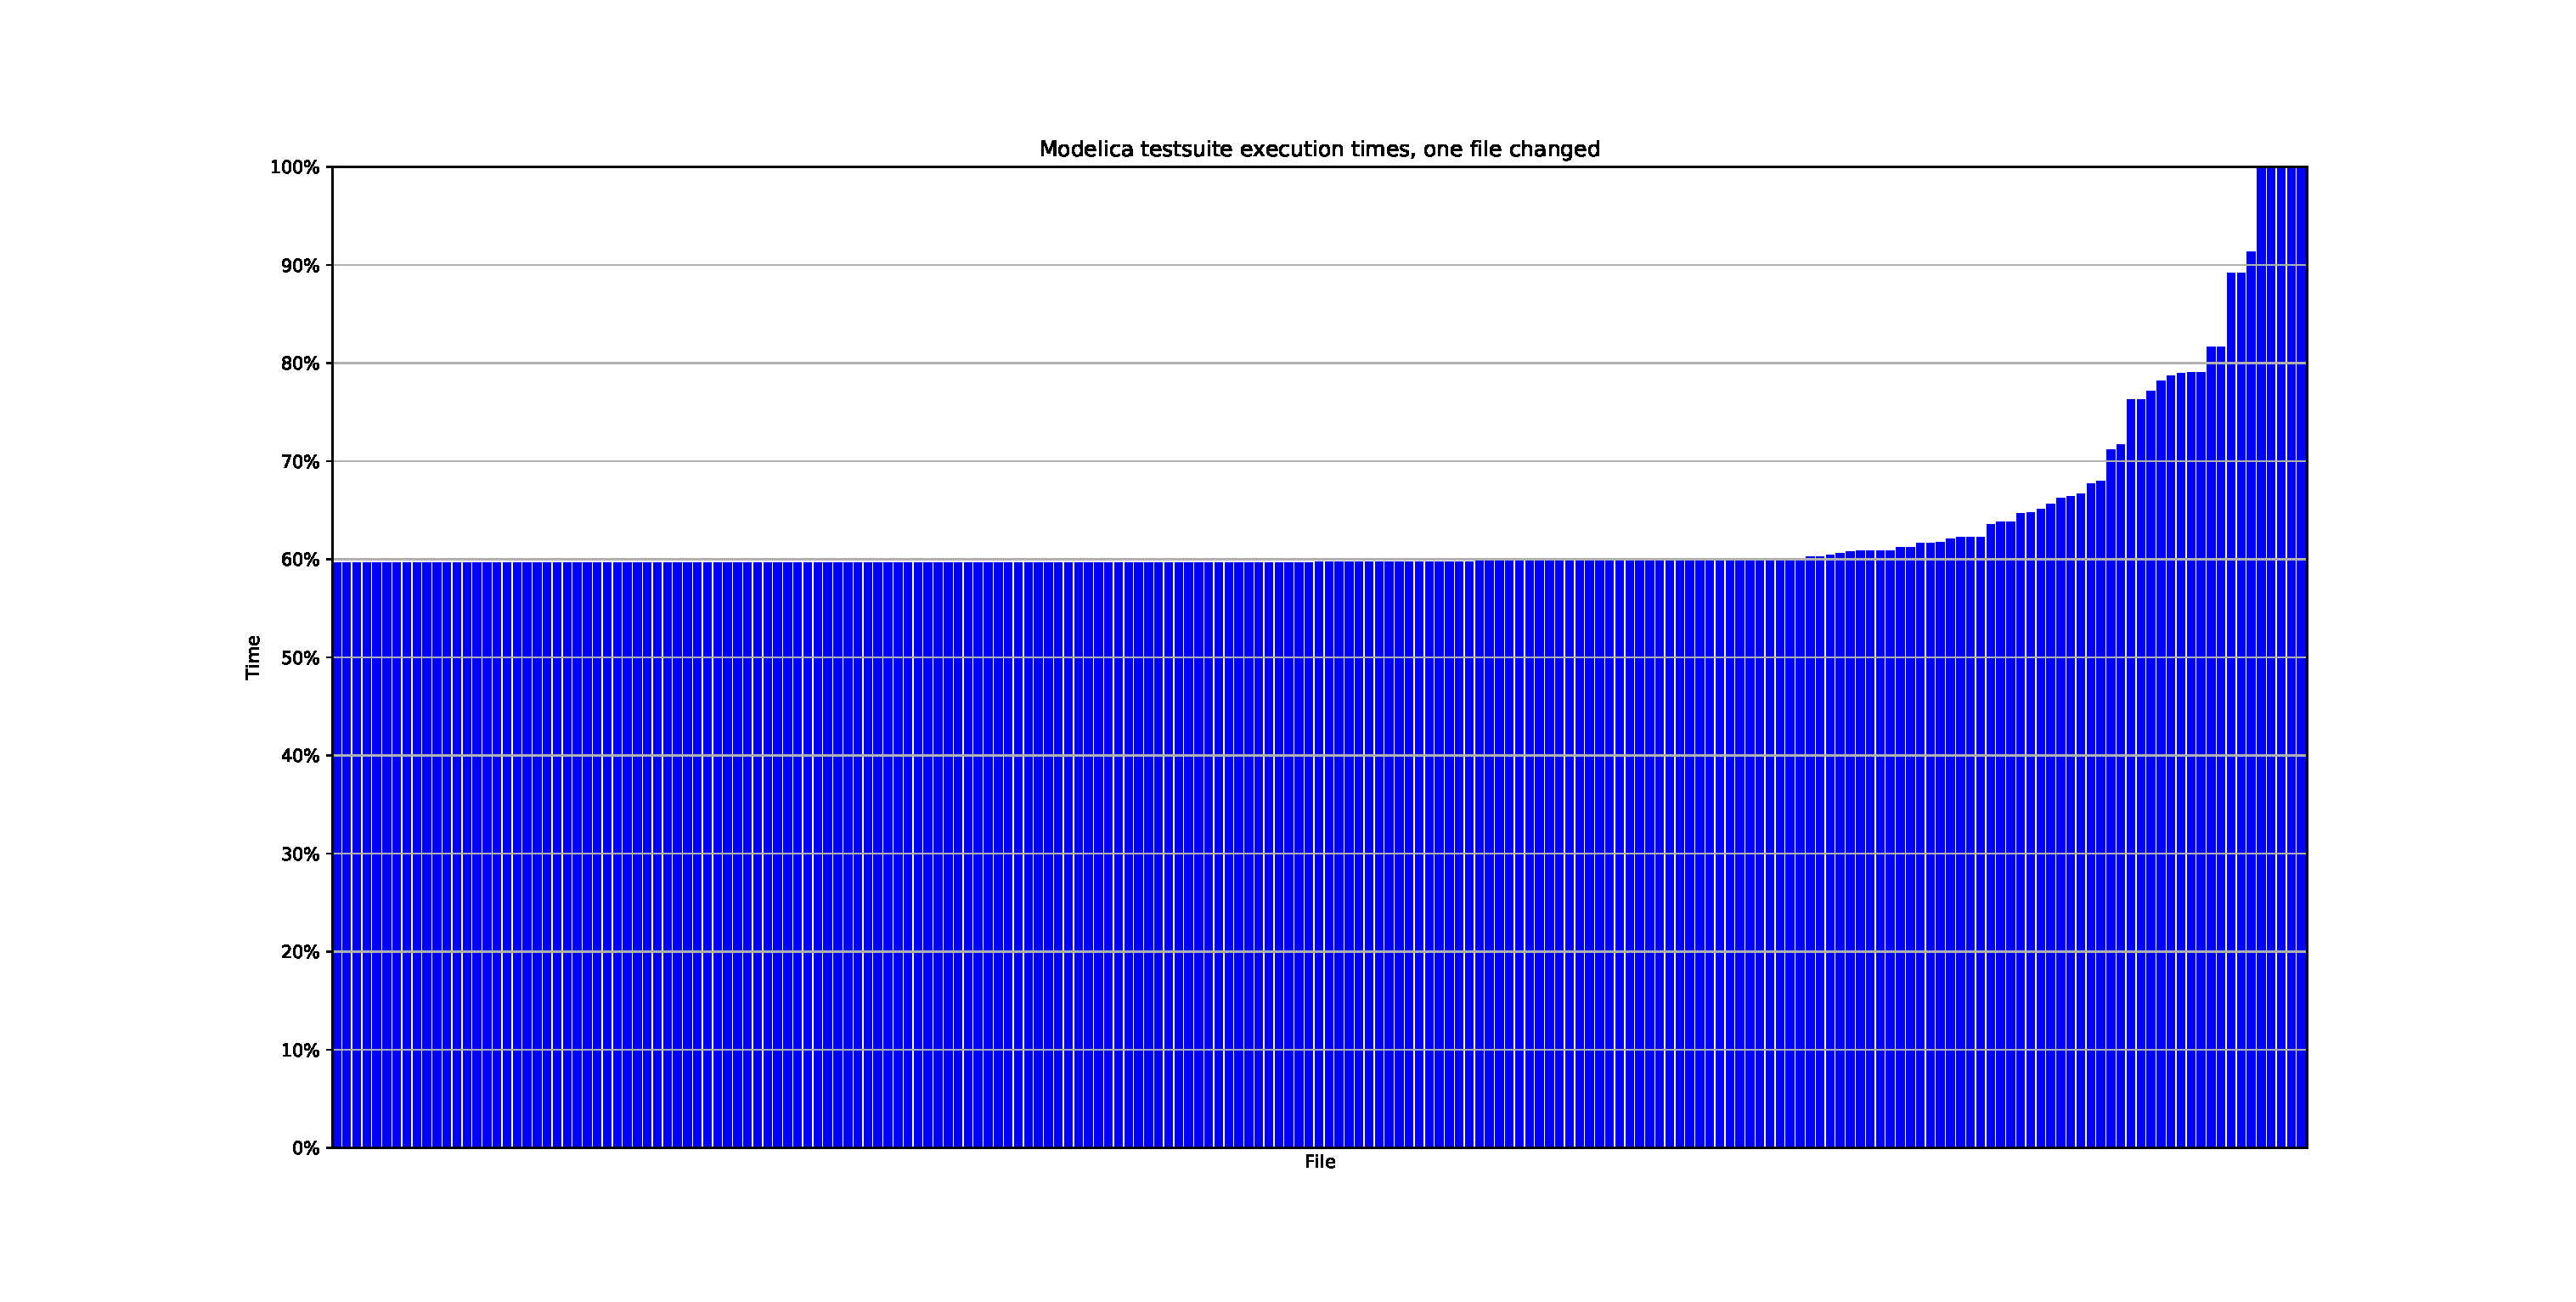
\includegraphics[width=1.5\textwidth]{EPS-graphs/one_file.eps}}
    \caption{One file changed.}
    \label{fig:onefile}
\end{figure}

\begin{figure}
    \centering
    \makebox[\textwidth][c]{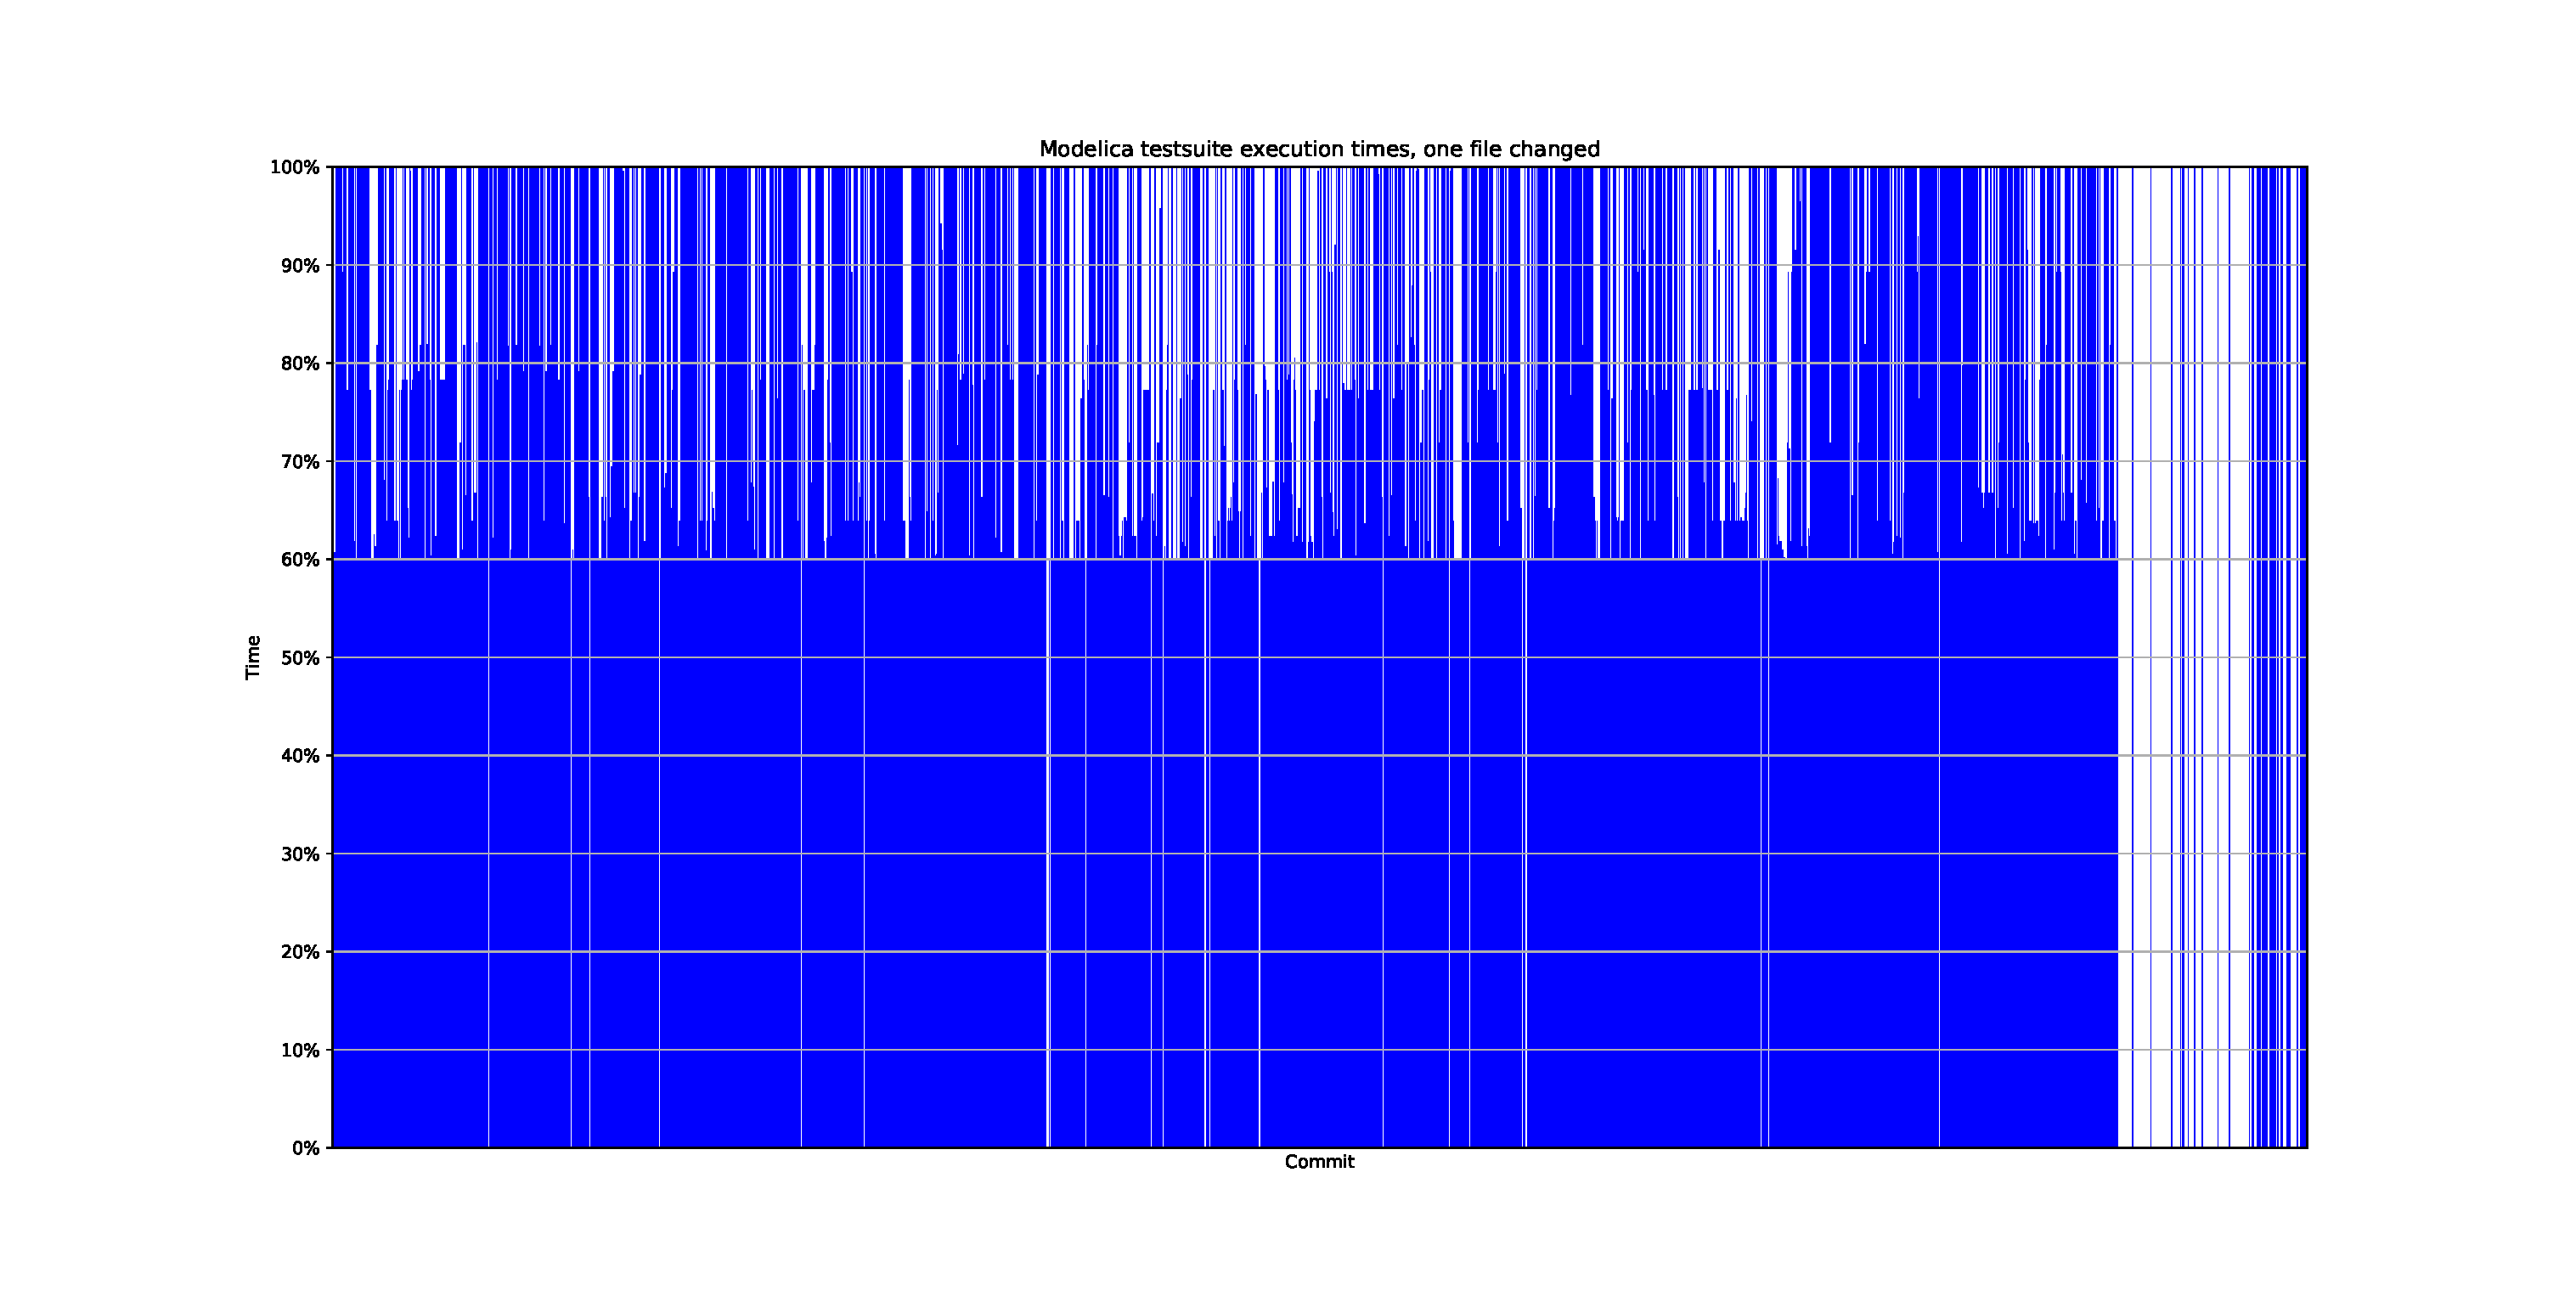
\includegraphics[width=1.5\textwidth]{EPS-graphs/history_plot.eps}}
    \caption{history plot for MSL.}
    \label{fig:mslhistory}
\end{figure}

\chapter[Future Work]{Future Work}
	
\chapter[Discussion]{Discussion}



\begin{itemize}
	\item Validity
	\item Analysis granularity
    \item Good and bad Modelica patterns for dependency analysis
\end{itemize}

\section{Related Work}

% Kan kanske flyttas till bakgrunden ev till test selection delen.
A master thesis similar to this one has previously been done at LTH. In the previously master thesis JastAdd was used to decrease the cost for testing of Android projects ~\cite{kampe2012dependroid}. There is research done on test selection. A method for safe RTS for Java has been developed before, that has many similarities with the method we are developing for Modelica. 

Studies have been conducted to investigate at which granularity dependency analysis pays off the most and how much percision it can have with out getting to expensive ~\cite{DBLP:conf/sigsoft/LegunsenHSLZM16}. It has also been done work in other techniques to achieve shorter time for testing, including dynamic test selection.

Det har tidigare gjorts ett liknande examensarbete på LTH. Där användes JastAdd för att minska kostnaden för testning av Android projekt. Det finns även forskning på området. Nästan precis samma sak som vi ska göra har gjorts tidigare men för Java ~\cite{DBLP:conf/pppj/OqvistHM16}. Utöver detta har det även tidigare undersökts hur finkornig en beroendeanalys kan vara utan att den blir för dyr ~\cite{DBLP:conf/sigsoft/LegunsenHSLZM16}. Det finns även arbete inom andra tekniker för att uppnå kortare test tider, till exempel dynamiskt testurval.
\chapter[Conclusion]{Conclusion}
\makebibliography{thebib}

\begin{appendices}
\chapter{About This Document}
\end{appendices}


\end{document}